\newpage
\section{User Stories}

Personas and User stories were populated and managed on a Trello board per Figure \ref{fig:user_stories_trello}.
Production stories are reproduced within this report for legibility.
Stories found to duplicate the intent of existing stories were ``binned''. 
A selection are visible within Figure \ref{fig:user_stories_trello}. For brevity, these stories are not presented within this report.

\begin{center}
	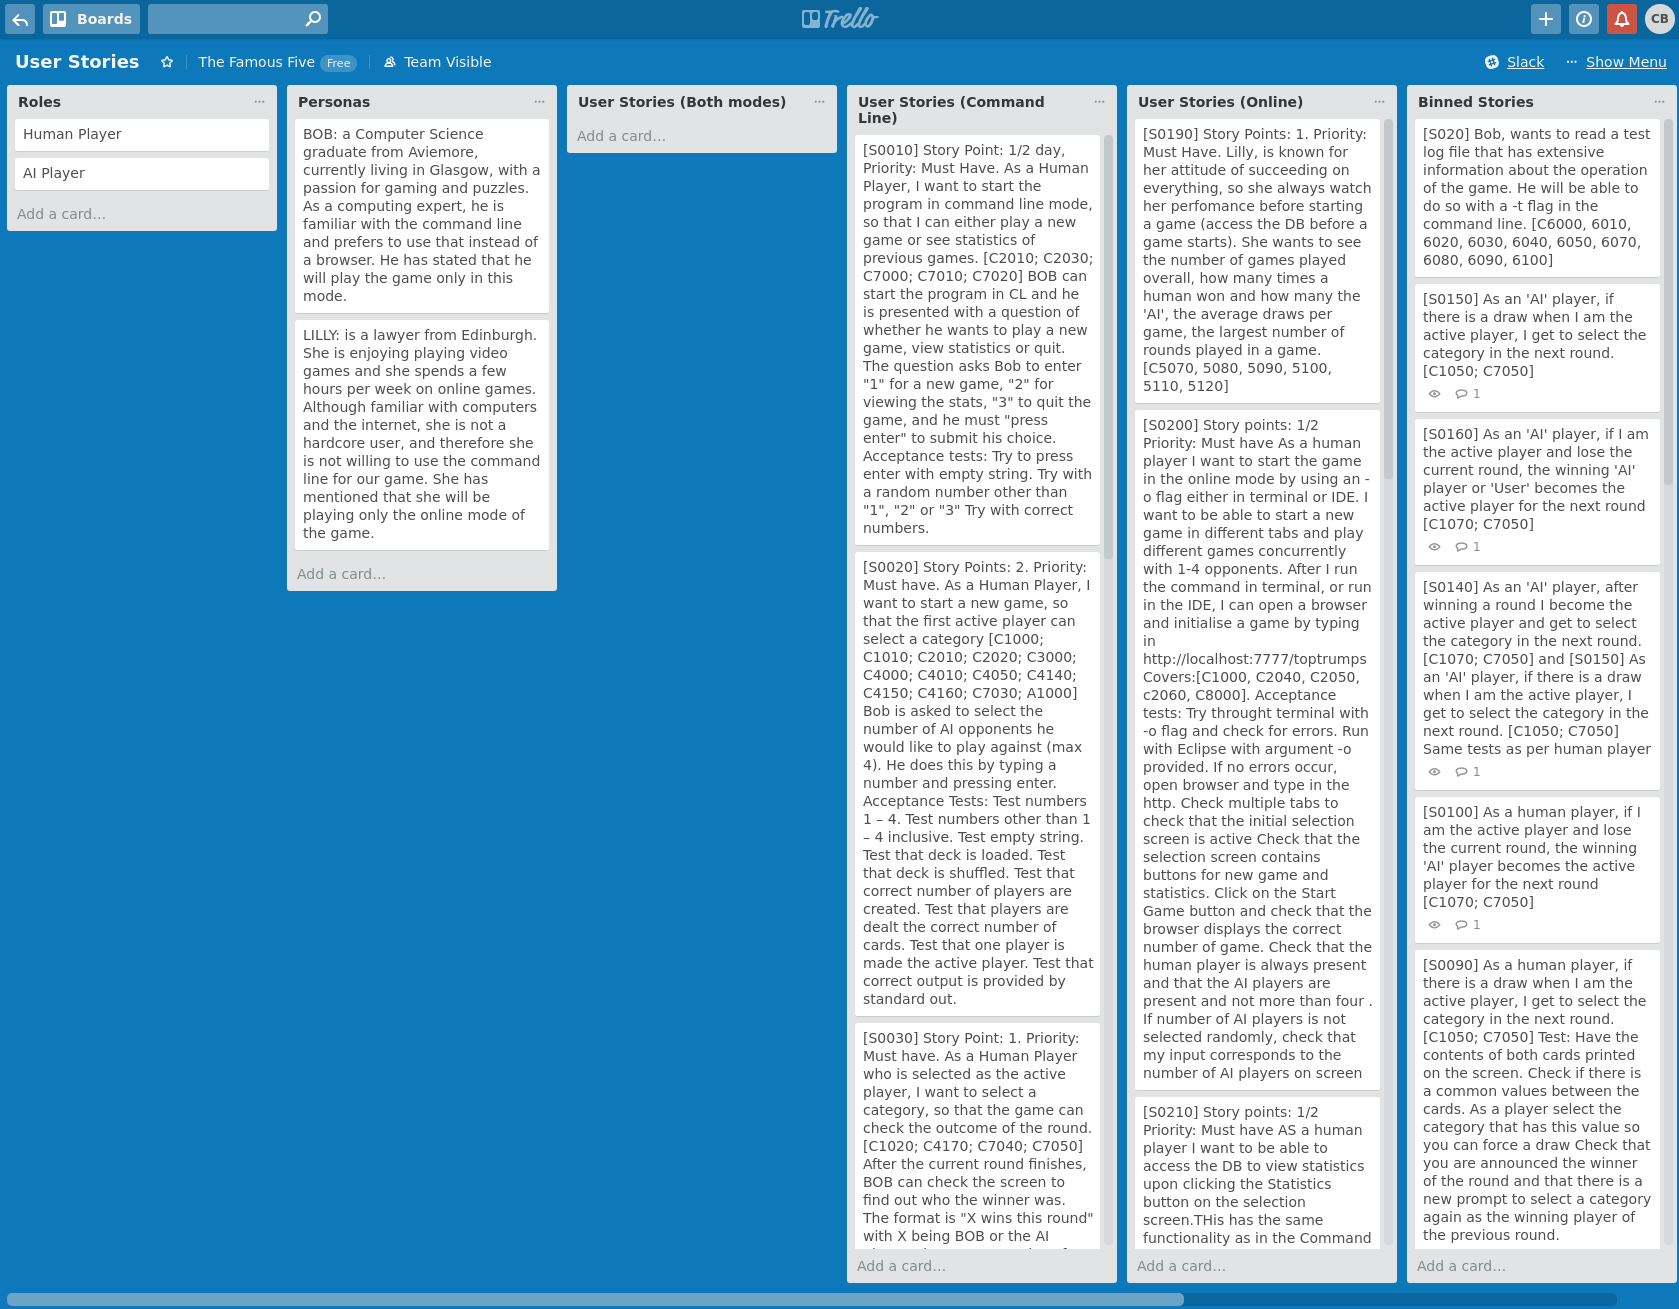
\includegraphics[scale=0.25]{user_stories_trello.png}
	\captionof{figure}{User Stories in Trello.}
	\label{fig:user_stories_trello}
\end{center}

\newpage
\subsection{Sprint \#1: Command Line Mode}
\bigskip

% ---------------------------------

\begin{card}{green}
{S0010}
{Must Have}
{Est: 1}
{Act: ?}
As a Human Player, I want to start the program in command line mode, so that I can either play a new game or see statistics of previous games.
\end{card}

\begin{card}{blue}
{S0010}{}{}{}
BOB can start the program in CL and he is presented with a question of whether he wants to play a new game, view statistics or quit. 
The question asks Bob to enter ``1'' for a new game, ``2'' for viewing the stats, ``3'' to quit the game, and he must ``press enter'' to submit his choice. Acceptance tests: Try to press enter with empty string. 
Try with a random number other than ``1'', ``2'' or ``3'' Try with correct numbers.
\end{card}

% ---------------------------------

\newpage

\begin{card}{green}
{S0020}
{Must Have}
{Est: 2}
{Act: ?}
As a Human Player, I want to start a new game, so that the first active player can select a category.
\end{card}

\begin{card}{blue}
{S0020}{}{}{}
Bob is asked to select the number of AI opponents he would like to play against (max 4). 
He does this by typing a number and pressing enter. 
Acceptance Tests: Test numbers 1 – 4. 
Test numbers other than 1 – 4 inclusive. 
Test empty string. 
Test that deck is loaded. 
Test that deck is shuffled. 
Test that correct number of players are created. 
Test that players are dealt the correct number of cards. 
Test that one player is made the active player. 
Test that correct output is provided by standard out.
\end{card}

% ---------------------------------

\newpage

\begin{card}{green}
{S0030}
{Must Have}
{Est: 1}
{Act: ?}
As a Human Player who is selected as the active player, I want to select a category, so that the game can check the outcome of the round.
\end{card}

\begin{card}{blue}
{S0030}{}{}{}
After the current round finishes, BOB can check the screen to find out who the winner was. 
The format is ``X wins this round'' with X being BOB or the AI player. 
The category values for each player are presented on the screen. 
Acceptance Tests: Play a round and check that the correct category values are shown for each player. 
Check that the correct player wins each time. Check that draw takes place if there are multiple highest cards. 
Check that correct player becomes/remains active player for next round. 
Check whether there is a message at the end specifying the winner.
\end{card}

% ---------------------------------

\newpage

\begin{card}{green}
{S0040}
{Must Have}
{Est: 1}
{Act: ?}
As a Human Player I want to know the outcome of the round, so that the game can progress to the next round.
\end{card}

\begin{card}{blue}
{S0040}{}{}{}
BOB will know if it is his or the opponents round without having to do anything further.
Tests: Check that after each round there is an output mentioning the winner. 
Check that user can continue to progress to new rounds even if eliminated.
\end{card}

% ---------------------------------

\newpage

\begin{card}{green}
{S0050}
{Must Have}
{Est: 1}
{Act: ?}
As a human player I want to choose to record game log information in a file when I start a game in command line mode.
\end{card}

\begin{card}{blue}
{S0050}{}{}{}
BOB can navigate to the game folder and see the game log. 
(Not sure if the user has the option NOT to log the game information) 
Acceptance Tests: Initiate a game and set -t flag in the CL. 
After the game finishes check that there exists a log file in the game directory, named topTrumps.log. 
Write a test log file with known content. 
RE-run the game and check that the original file is overwritten with the correct content. 
Check the content of the file as per C6030- C6100 requirements.
\end{card}

% ---------------------------------

\newpage

\begin{card}{green}
{S0130}
{Must Have}
{Est: 1}
{Act: ?}
As a Human Player, when not the active player for a round, I want the active AI player to select a single category which has the highest or joint highest value for their topmost card.
\end{card}

\begin{card}{blue}
{S0130}{}{}{}
While developing, have the system.out print all the values for the AI player, i.e. the contents of their top most card. 
Upon selecting a category, have a system.out for the category selected and the value. 
Compare with the contents of the whole card to make sure that the highest value category is always selected by the AI player.
\end{card}

% ---------------------------------

\newpage

\begin{card}{green}
{S0180}
{Must Have}
{Est: 1}
{Act: ?}
Bob and Lilly are really into statistics and they want to keep track of the game stats after a game ends. 
As experienced players they want to know how many draws were in the game, how many rounds were played, how many rounds were won by each player (with clear indication) and who won the game. 
They don't want to press anything for this procedure, it must be automated.
\end{card}

\begin{card}{blue}
{S0180}{}{}{}
Query the Database to make sure everything has been recorded.
\end{card}

% ---------------------------------

\newpage
\subsection{Sprint \#2: Online Mode}
\bigskip

\begin{card}{green}
{S0190}
{Must Have}
{Est: 1}
{Act: ?}
Lilly, is known for her attitude of succeeding on everything, so she always watch her performance before starting a game (access the DB before a game starts). 
She wants to see the number of games played overall, how many times a human won and how many the ``AI'', the average draws per game, the largest number of rounds played in a game.
\end{card}

\begin{card}{blue}
{S0190}{}{}{}
?
\end{card}

% ---------------------------------

\newpage

\begin{card}{green}
{S0200}
{Must Have}
{Est: 1}
{Act: ?}
As a Human Player, I want to start the game in the online mode by using an -o flag either in terminal.  
I want to be able to start a new game in different tabs and play different games concurrently with 1-4 opponents. 
After I run the command in terminal, I can open a browser and initialise a game by typing in http://localhost:7777/toptrumps.
\end{card}

\begin{card}{blue}
{S0200}{}{}{}
Try in terminal with -o flag and check for errors. 
If no errors occur, open browser and type in the http.
Check multiple tabs to check that the initial selection screen is active Check that the selection screen contains buttons for new game and statistics.
Click on the Start Game button and check that the browser displays the correct number of game. 
Check that the human player is always present and that the AI players are present and not more than four. 
If number of AI players is not selected randomly, check that my input corresponds to the number of AI players on screen.
\end{card}

% ---------------------------------

\newpage

\begin{card}{green}
{S0210}
{Must Have}
{Est: 1}
{Act: ?}
As a Human Player, I want to be able to access the DB to view statistics upon clicking the Statistics button on the selection screen.
This has the same functionality as in the Command Line mode as described in [S0180].
The difference is the way I will access this functionality.
\end{card}

\begin{card}{blue}
{S0210}{}{}{}
Check that the Statistics button is responsive. 
How the data will be presented in the Online mode???????
Check that all games are stores to the DB, I.e all instances as represented by different tabs.
\end{card}

% ---------------------------------

\newpage

\begin{card}{green}
{S0220}
{Must Have}
{Est: 1}
{Act: ?}
As a Human Player, I want to be able to see that the game has actually started, and be guided through the steps of what I need to do next. 
I want to be able to have access on the game information that allow me to navigate through it, and be presented with my options if I am the active player, or have a visual on the storyline if an AI is the active player.
\end{card}

\begin{card}{blue}
{S0220}{}{}{}
After clicking on the new game button check that the screen shows: Confirmation that the game has started, by showing for example ``Deck has been shuffled and dealt''.
The round number I am currently playing Who the active player is.
Check that I have the number of cards I have in hand, either on the card, or somewhere else on screen.
My topmost card with the characteristics' values.
A button that allows me to proceed to the next step. 
That is, to select my category if I am the active player or make the AI plaeyer select his. 
Check that if I am not the active player I do not have the option to select my category.
\end{card}

% ---------------------------------

\newpage

\begin{card}{green}
{S0230}
{Must Have}
{Est: 1}
{Act: ?}
As a Human Player, and after I have selected to proceed with the game after selecting the button as described by S0220, I want  to trigger the current round.
I want to be able to select my category as an active player, or ``notify'' the AI player that he needs to do the same, and in the end I would like to know the outcome of the round.
\end{card}

\begin{card}{blue}
{S0230}{}{}{}
If I am the active player: Check that the button makes me select a category by poping a drop down menu or similar. 
Check that selecting my category the game proceeds to next step If I am not the active player. 
Check that the game continies by having the AI player selecting category.
In both cases: After selection, check that I have the option to go to the next step, I.e. show the winner After the category selection, check that all cards with their values are visible on screen and that the winner is mentioned. 
Check that the same winner has the privilege of selecting the new category Check that the number of available cards in hand have been recalculated.
\end{card}

% ---------------------------------

\newpage

\begin{card}{green}
{S0240}
{Must Have}
{Est: 2}
{Act: ?}
As a Human Player, I want to have access to the game information if a draw has occurred. 
That includes to be aware that the outcome was a draw and the volume of the communal. 
I want to be able to re-select if I was the winner of the previous round. 
\end{card}

\begin{card}{blue}
{S0240}{}{}{}
Check that in the case of a draw, the screen shows that clearly. 
Next check that there is an indication of the number of cards in the communal pile Check that a button is present, allowing me to order the game to proceed to the next round. 
Check that the round number has increased by 1 after the draw and after I have selected to go on. 
Check that the category selector from previous round is the current selector. 
In the first winning case, display the number of cards in communal pile to make sure it is reset.
\end{card}

% ---------------------------------

\newpage

\begin{card}{green}
{S0250}
{Must Have}
{Est: 1}
{Act: ?}
As a Human Player, I want to know who the overall winner was.
\end{card}

\begin{card}{blue}
{S0250}{}{}{}
Check that when the last round is finished, the name of the winner is shown. 
Have a summary of winning rounds as per video example???? TO DISCUSS.
Make sure there is a button to return me to the selection screen, from where I can access the DB or play new game.
\end{card}

% ---------------------------------

% \newpage

% \begin{card}{green}
% {S?}
% {?}
% {Est: ?}
% {Act: ?}
% ?
% \end{card}

% \begin{card}{blue}
% {S?}{}{}{}
% ?
% \end{card}